\documentclass[sigconf]{acmart}

\usepackage{booktabs} % For formal tables
\usepackage{amsmath,amssymb,amsthm}
\usepackage{graphicx}

%\newtheorem{theorem}{Theorem}
%\newtheorem{corollary}{Corollary}[theorem]
%\newtheorem{lemma}{Lemma}
\newtheorem{case}{Case}

\usepackage[colorinlistoftodos]{todonotes}
\usepackage{pgfplots} 
\usepackage{amsmath}

%\usepackage{microtype}%if unwanted, comment out or use option "draft"

%\graphicspath{{./graphics/}}%helpful if your graphic files are in another directory

% Copyright
%\setcopyright{none}
%\setcopyright{acmcopyright}
%\setcopyright{acmlicensed}
\setcopyright{rightsretained}
%\setcopyright{usgov}
%\setcopyright{usgovmixed}
%\setcopyright{cagov}
%\setcopyright{cagovmixed}


% DOI
\acmDOI{10.475/123_4}

% ISBN
\acmISBN{123-4567-24-567/08/06}

%Conference
\acmConference[EMSOFT'17]{ACM SIGBED International Conference on Embedded Software}{October 2017}{Seoul, South Korea} 
\acmYear{2017}
\copyrightyear{2017}

\acmPrice{15.00}

\newcommand{\IL}[1]{$\spadesuit$\footnote{IL: #1}}

\begin{document}
	\title{Data Freshness Over-Engineering: Formulation and Basic Results}
	%\titlenote{Produces the permission block, and
	%	copyright information}
	%\subtitle{Extended Abstract}
	%\subtitlenote{The full version of the author's guide is available as
	%	\texttt{acmart.pdf} document}
	
	
	\iffalse
	\author{Dagaen Golomb}
	%\authornote{Dr.~Trovato insisted his name be first.}
	\orcid{0000-0002-1892-4098}
	\affiliation{%
		\institution{University of Pennsylvania}
		%\streetaddress{P.O. Box 1212}
		\city{Philadelphia} 
		\state{Pennsylvania} 
		\postcode{19104}
	}
	\email{dgolomb@seas.upenn.edu}
	
	\author{Deepak Gangadharan}
	%\authornote{The secretary disavows any knowledge of this author's actions.}
	\affiliation{%
		\institution{University of Pennsylvania}
		%\streetaddress{P.O. Box 1212}
		\city{Philadelphia} 
		\state{Pennsylvania} 
		\postcode{19104}
	}
	\email{deepakg@seas.upenn.edu}
	
	\author{Sanjian Chen}
	%\authornote{This author is the one who did all the really hard work.}
	\affiliation{%
		\institution{University of Pennsylvania}
		%\streetaddress{P.O. Box 1212}
		\city{Philadelphia} 
		\state{Pennsylvania} 
		\postcode{19104}
	}
	\email{sanjian@seas.upenn.edu}
	
	\author{Oleg Sokolsky}
	\affiliation{%
		\institution{University of Pennsylvania}
		%\streetaddress{P.O. Box 1212}
		\city{Philadelphia} 
		\state{Pennsylvania} 
		\postcode{19104}
	}
	\email{sokolsky@cis.upenn.edu}
	
	\author{Insup Lee}
	\affiliation{%
		\institution{University of Pennsylvania}
		%\streetaddress{P.O. Box 1212}
		\city{Philadelphia} 
		\state{Pennsylvania} 
		\postcode{19104}
	}
	\email{lee@cis.upenn.edu}
	
	% The default list of authors is too long for headers}
	\renewcommand{\shortauthors}{D. Golomb et al.}
	\fi
	
	\begin{abstract}
		In many application scenarios, data consumed by real-time tasks are required to meet some form of maximum age requirement, or freshness guarantee. In this paper, we consider the end-to-end freshness constraint of data that is passed along a chain of tasks in a uniprocessor setting. We do so with few assumptions regarding the scheduling algorithm used. We present a method for selecting the periods of the tasks in chains of length two and three such that the end-to-end freshness requirement is satisfied, and then extend our method to arbitrary chains. We perform evaluations of both methods using parameters from an embedded benchmark suite (E3S) and several schedulers to support our result.
	\end{abstract}

	%
	% The code below should be generated by the tool at
	% http://dl.acm.org/ccs.cfm
	% Please copy and paste the code instead of the example below. 
	%
	
	\begin{CCSXML}
		<ccs2012>
		<concept>
		<concept_id>10010520.10010570</concept_id>
		<concept_desc>Computer systems organization~Real-time systems</concept_desc>
		<concept_significance>500</concept_significance>
		</concept>
		</ccs2012>
	\end{CCSXML}
	
	\ccsdesc[500]{Computer systems organization~Real-time systems}
	
	% We no longer use \terms command
	%\terms{Theory}
	
	\keywords{Real-time, freshness, optimization}
	
	
	\maketitle

	\section{Introduction}

There are many applications where a task needs to consume data in order to perform its duties. In real-time systems, this input is often sensor data that is crucial for determining the behavior of the system. Input may also be from the output of other tasks. In these types of systems, there is usually an explicit or implicit timeliness requested for this data. The relevance of a computation can be intuitively evaluated by the age, or "freshness," of the data that was used during the computation.

Traditionally, tasks have been over-engineered to provide fresh data. Imagine a task that must perform some computation on data, produced by another task, every one second. Should the task producing the required data run every second? 500 milliseconds? 100 milliseconds? How is the designer to decide? In these situations, engineers may err on the side of caution and choose to produce the input data faster than necessary, which they then need to test in order to evaluate safety. For example, A task that reads a sensor value and forwards it to another task may be dispatched fifty times a second even though the consuming task only needs data younger than one tenth of a second for safety. While this is presumably safe, it reduces the efficiency (and possibly schedulability) of the system, and there is no formal method for us to decide if this value is safe regardless. This leads to more dependence on testing. As Microsoft acknowledges, overenginnering alway leads to wasted effort \cite{CODEMINE}. This often leads to several cycles of parameter tuning in order to ensure the safety and efficiency of the system without ultimately guaranteeing optimal efficiency, as noted by several others in the field \cite{BiniNatale,SetoLehoczkySha,ChantemWangLemmonHu,BelwalCheng}. This paper outlines a formalization of this over-engineering strategy and presents results for choosing the period of input tasks given little information about the underlying system.
	\section{Formalization}

\subsection{Task Definitions}

Our model assumes a periodic task set on a unicore system. For periodic task sets, each task $A$ is characterized by a period $P_A$, a relative deadline $D_A$, and a worst-case execution time (WCET) $E^u_A$. We additionally include a best-case execution time (BCET) $E^l_A$.

A job is an instance of a task, i.e. one of the actual executions of a task. Each task produces multiple jobs and in the periodic model, a job is released every $P_A$ time. Each $i^{th}$ job of task $A$ has a release time $r^i_A$ and a finish time $f^i_A$. Note that $f^i_A - r^i_A$ is lower bounded by BCET (when the task is executed immediately and runs to completion) but not upper bounded by the WCET if the job can be preempted. However, assuming the system is schedulable, the job is completed before the its deadline. If this is not the case then the job has experienced a deadline miss. In this work we will consider deadlines to be equal to periods for simplicity and clarity, but our model could be extended to account for other deadlines.

Since we wish to uphold a data freshness guarantee, we define $d_{A \to B}$ to be the desired upper bound on data freshness for data produced by task $A$ and consumed by task $B$. Lastly, we define a value that will help us formulate the requirements of our system. Let $C_A(r^i_B)$ denote the most recently completed job of task $A$ before the release of job $i$ of task $B$. This will be useful since we assume the most recently produced output from a task is the freshest. This assumption holds because of our period = deadline assumption, but is also easily enforced if that assumption is removed.

\subsection{Communication Definitions}

We include communication, storage, or other latencies into our formulation. For our purposes, data latency denotes any delay in storing or transferring a value to another task. Examples include the delay to store a value in a database, inter-processor communication, and network delays. For our formulation, we require the following values to be provided: Minimum Data Delay $DL^{min}$ and Maximum Data Delay $DL^{max}$.

Since our formulation will consider data to be available at task completion, we can abstract the communication delay into our task execution times as follows:

\begin{center}
		$E^{l,min}_A = E^l_A + DL^{min}$ \text{ and } $E^{u,max}_A = E^u_A + DL^{max}$
\end{center}

\subsection{Assumptions}

Since we do not know the nature of the tasks, particularly when they produce and consume data, we choose to abstract the specifics of data production and consumption. We assume tasks consume data at the very beginning of their execution as this enacts the strictness (shortest) freshness deadline. Since execution could happen immediately at release time, without knowledge of the scheduler, we assume jobs read input values at the time of their release.

On the other hand, we assume data is produced at finish time. Therefore, we must wait until the completion of a job before we can consider its data available, at which time it overwrites the data from the last completed job of the task. While we do not consider delay from the polling task, collection tasks are often small and we consider this trivial. If the initial task has non-trivial execution time its WCET can be subtracted from the desired freshness bound. While producing at the end of a task does not produce the worst staleness, it is easy to hold off production until the end of task and, similarly to the polling task mentioned in the last sentence, one can subtract the difference between the end of a job and the earlies it could produce data from the freshness constraint.

Since the freshness of the final, fully-transformed data is often of interest, we assume that the period of the final consuming task is fixed, i.e., if a designer wants the transformed data to be at most 50 milliseconds old, it is intuitive that they would select this as the period of the final task. We will assume the designer selects an appropriate period for this task and would like to compute the input tasks' periods to meet their freshness requirement. In this work we present our approach considering unicore systems, but will show how the work seamlessly applies to multicore systems.

\subsection{Requirements}

Using the notation and assumptions above, for a producer ($A$) and consumer ($B$) pair we define the freshness requirement of data produced by task $A$ and consumed by job $i$ of task $B$ as follows:
\begin{center}
	$\forall i, r^i_B - f_A^{C_A(r^i_B)} \leq d_{A \to B}$
\end{center}
That is, at the release of any job $i$ of task $B$, the time since the completion of the last job by task $A$ is less than or equal to the freshness bound $d_{A \to B}$.


\subsection{Problem Statement}

The problem statement is as follows. Let $E^{*,*}_k$ denote that we have both worst-case and best-case execution times including communication and other latencies for task $k$, and let $U(T)$ denote the system utilization. We have $n$ tasks in the chain.

\iffalse
\begin{equation*}
	\begin{aligned}
		& \text{Given}
		& & E^{*,*}_A, E^{*,*}_B, P_B, \text{ and } d_{A \to B} \\
		& \text{Find}
		& & P_A \\
		& \text{That Minimizes}
		& & U(T) = \sum_i \frac{E_i^{u,max}}{P_i}\\
		& \text{Subject To}
		& & \forall i, r^i_B - f_A^{C_A(r^i_B)} \leq d_{A \to B}
	\end{aligned}
\end{equation*}
\fi

\begin{equation*}
	\begin{aligned}
		& \text{Given}
		& & \forall k, E^{*,*}_k; \text{ and } d_{1 \to n} \\
		& \text{Find}
		& & \forall k < n, P_k \\
		& \text{That Minimizes}
		& & U(T) = \sum_n \frac{E_n^{u,max}}{P_n}\\
		& \text{Subject To}
		& & \forall i, \sum_{j=2}^{n} (r^i_j - f_{j-1}^{C_j(r^i_{j-1})}) + \sum_{j=2}^{n-1} E_n^{u,max} \leq d_{1 \to n}
	\end{aligned}
\end{equation*}

Expressed textually, we minimize utilization while keeping the sum of task WCETs between the original producer and the final consumer plus the sum of any time spent between the end of a job of task $A$ and the release of a job of the next task $B$, to be less than our freshness bound. This quantity is the total time the data spends in flight. We use WCETs since this case produces the most strict local deadlines, which we describe later, for each pair of tasks.

We do not consider schedulability in the formulation as to maintain maximum generality. Therefore, our solution will not guarantee schedulability, which must be confirmed using algorithm-specific methods afterwards. However, our solution relies on an assumption of the schedulability of the final task set and is thereby invalidated if this is not the case.

It is clear this minimization has a solution. Assume all periods are low enough to ensure the freshness bound (all close to $0$ for example, as it is clear all periods arbitrarily close to $0$ would cause the bound to hold). We can lower utilization by increasing any $P_k$, but at some point increasing $P_k$ will violate our freshness bound. For example, if $P_k = 2 \cdot d_{1 \to n}$ freshness will not hold, while setting $P_k$ arbitrarily closer to $0$ will cause the bound to hold (disregarding schedulability). At some point between these two the system switches between upholding and violating the freshness bound. This point is one solution.
	\section{Two Task Result}

First we consider the simplest case where there are only two tasks: one producing a value (task $A$) and one consuming it (task $B$). Considering just task $A$ we can see the worst case depicted in Figure~\ref{fig:2Tasks}. This scenario assumes schedulability to ensure that one job of $A$ must run and complete within each period. This is where our schedulability assumption becomes vital for our solution.

\begin{figure}[h]
	\centering
	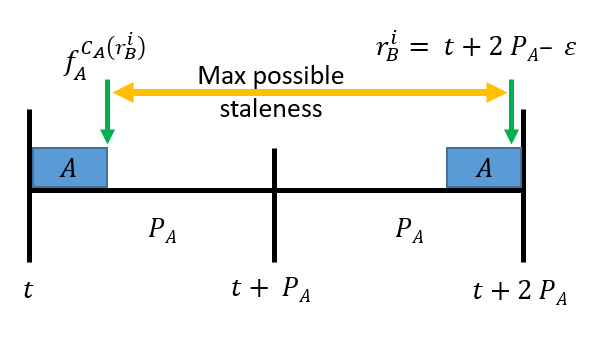
\includegraphics[width=0.3\textwidth]{figures/2TaskMaxStaleness}
	\caption{Maximum Staleness Scenario for Data from Task A.}
	\label{fig:2Tasks}
\end{figure}

Figure \ref{fig:2Tasks} labels the maximum separation between two publishes of output data from the depicted task. To maximize the staleness, we assume a job of task $B$ is released arbitrarily close to the finish of the second job of task $A$ and that the first (BCET) job of task $A$ ran to completion at the beginning of the previous period.

Note that we assume deadlines are equal to periods. However, it is easy to see here that a shorter deadline moves the latest possible execution of the second job of task A earlier, and hence decreases the max possible staleness. We will not consider this case further but it will be clear later how this could be substituted in place of our equal period and deadline example.

\begin{theorem}
	\label{thm:2TaskMaxWaiting}
	The scenario in Figure~\ref{fig:2Tasks} is the upper bound scenario for data freshness for data produced by a task.
\end{theorem}

\begin{proof}
	Note that one job must be executed within each period as per the definition of periodic tasks and our assumption of task set schedulability. Consider any placement of two jobs of a task within two consecutive periods. Assume this instance is not the one depicted in Figure~\ref{fig:2Tasks}. Then at least one of the following apply:
	\begin{case}
		The job in the first period is not completed as soon as possible. In this case, move the start of this job execution $\epsilon$ earlier. This increases the staleness by $\epsilon$.
	\end{case}
	\begin{case}
		The job in the second period is not completed as late as possible. In this case, move the start of this job execution $\epsilon$ later. This increases the staleness by $\epsilon$.
	\end{case}
	Since all other instantiations of the problem can be moved closer to the depicted instance while strictly increasing data staleness, it follows that the depicted instance is the unique worst case for output data staleness.
\end{proof}

Now that we have proven the above scenario is the worst case with regards to the freshness of data from task $A$, we can use algebra to solve for the constraint on $P_A$. From Figure~\ref{fig:2Tasks} we can see that the maximum staleness is composed of two periods of $A$ less one execution time of $A$ less $\epsilon$. We want this to be less than our freshness bound $d_{A \to B}$. We can then solve for $P_A$ to prove the following lemma.

Note that we assume the best case execution time and data delay for the first job in order to maximize staleness. The execution time of the second job is irrelevant.

\begin{lemma}
	\label{lem:2TaskResult}
	To ensure the output of task $A$ is always at most $d_{A \to B}$ old, choose $P_A \leq \frac{d_{A \to B} + E^{l,min}_A}{2}$.
\end{lemma}

\begin{proof}
	\begin{align*}
		d_{A \to B}&\geq 2P_A-E^{l,min}_A-\epsilon &\mbox{From Figure \ref{fig:2Tasks}}&\\
		P_A&\leq \frac{d_{A \to B} + E^{l,min}_A + \epsilon}{2} &\mbox{Rearrange}&\\
		P_A&\leq \frac{d_{A \to B} + E^{l,min}_A}{2} &\mbox{$\epsilon \to 0$}&
	\end{align*}
\end{proof}

We can justify bringing epsilon to zero as this is decreasing the period value and hence strictly increasing freshness. Thus if we set $P_A$ equal to the the above quantity we ensure that the output of task $A$ is always at most $d_{A \to B}$ old, and therefore can never be older when consumed by task $B$. We can also set $P_A$ less than this quantity and maintain the freshness guarantee.

Recall that our fitness metric is total utilization. It is trivial to see that choosing $P_A$ as large as possible will minimize the task set utilization. Thus the solution for the two task scenario while minimizing utilization is to set $P_A$ equal to the quantity in the lemma.

	\section{Three Task Result}

We now extend the above idea to three tasks. In this scenario, let our tasks be denoted as $A$, $B$, and $C$. Task $A$ produces output consumed by task $B$, which in turn produces output consumed by task $C$. We want to limit the age of the output of $A$ that is eventually used by $C$.

For this scenario, define $d_{A \to C}$ as the maximum age of the data produced by task $A$ that is used by task $C$. Note that we are not making any assumptions about when a job of task $B$ is executed between jobs of tasks $A$ and $C$. The formalization is similar to the two task scenario:

\begin{equation*}
	\begin{aligned}
		& \text{Given:}
		& & E^{*,*}_A, E^{*,*}_B, E^{*,*}_C, P_C \text{ and } d_{A \to C} \\
		& \text{Find:}
		& & P_A \text{ and } P_B \\
		& \text{That Minimizes:}
		& & U(T) = \sum_i \frac{E_i^{u,max}}{P_i} \\
		& \text{Subject To:}
		& & 
	\end{aligned}
\end{equation*}
\begin{equation*}
	\forall i, r^i_C - f_B^{C_B(r^i_C)} + E^{u,max}_B + r_B^{C_B(r^i_C)} - f_A^{C_A(r_B^{C_B(r^i_C)})} \leq d_{A \to C}
\end{equation*}

\noindent Note that we assume worst case execution and data delay for task $B$. This will produce a more urgent local deadline that will enforce freshness also when this does not occur. More rigorously, let $\delta = E_B^{u,max} - E_B^{l,min}$. Using the max value as we do instead of the least value decreases $d_{B \to C}$ by $\delta$. As can be seen from Lemma~\ref{lem:2TaskResult} this decreases $P_B$ by $\delta / 2$. Viewing task $B$ and $C$ alone as their pair, it is easier to see that the freshness is made of two periods of $B$ for a total decrease of $\delta$. Hence, in the case of minimal execution of task $B$ the execution increases by $\delta$ but this same amount has already been compensated for in the formulation.

The execution of the three tasks is outlined in the figure \ref{fig:3Tasks}.

\begin{figure}[!ht]
	\centering
	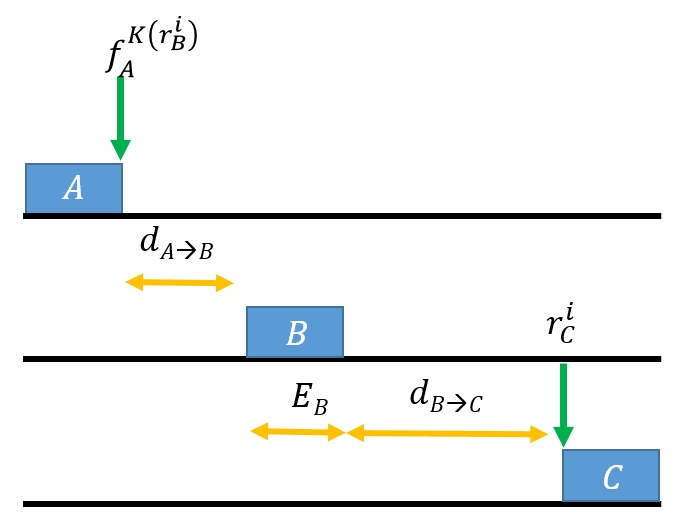
\includegraphics[width=0.3\textwidth]{figures/3TaskMaxStaleness}
	\caption{Maximum Staleness Scenario for Data from Task A.}
	\label{fig:3Tasks}
\end{figure}

Figure~\ref{fig:3Tasks} labels the several intervals in the execution of the three tasks. Note how between tasks $A$ and $B$ and between tasks $B$ and $C$ we've added local freshness constraints. By meeting these two freshness constraints, the freshness of data from task $A$ to task $C$ is ensured. These added constraints will not be present in our final solution but are added here to allow us to introduce Lemma~\ref{lem:2TaskResult} while considering task $B$. These local constraints are used as free variables in our optimization, and once determined we will use our lemma to calculate period assignments that rely only on the end-to-end constraint and task execution times.

From Figure~\ref{fig:3Tasks} we can see that the maximum age of the data from task $A$ used by task $C$, $d_{A \to C}$, is the sum of three values. Concretely,

\begin{center}
	$d_{A \to C} = d_{A \to B} + E^{u,max}_B + d_{B \to C}$
\end{center}

We now use our lemma to extend the two task result to this scenario. Using Lemma \ref{lem:2TaskResult}\ldots

\begin{center}
	$P_A \leq \frac{d_{A \to B} + E^{l,min}_A}{2} \text{ and } P_B \leq \frac{d_{B \to C} + E^{l,min}_B}{2}$
\end{center}

Our lemma uses the BCET for the first task in each pair in order to maximize the possible staleness. For our freshness guarantee, we will use the BCET to be pessimistic with the data age, whereas when calculating utilization we will use the WCET. That is, our solution will ensure freshness even in with best-case execution of the first task, while minimizing the maximum utilization the system could experience.

We simplify the objective by removing constants from the utilization expression and then transform it by substituting from Lemma~\ref{lem:2TaskResult}, using equality since lower periods increase utilization:

\begin{align*}
	U(T) &= \left(\frac{E^{u,max}_A}{P_A} + \frac{E^{u,max}_B}{P_B}\right) &\mbox{Objective}&\\
	&= \left(\frac{E^{u,max}_A}{\frac{d_{A \to B} + E^{l,min}_A}{2}} + \frac{E^{u,max}_B}{\frac{d_{B \to C} + E^{l,min}_B}{2}}\right) &\mbox{Substitution}&\\
	&= \frac{2E^{u,max}_A}{d_{A \to B}+E^{l,min}_A} + \frac{2E^{u,max}_B}{d_{B \to C}+E^{l,min}_B} &\mbox{Simplification}&
\end{align*}

We minimize this objective to arrive at the following solution.

\begin{theorem}
	\label{thm:3TaskResult}
	Given $E^{*,*}_A$, $E^{*,*}_B$, $E^{*,*}_C$, and $P_C$, to minimize utilization while enforcing the freshness bound $d_{A \to C}$, choose
	\begin{align*}
		P_A &= \frac{\sqrt{\frac{E^{u,max}_A}{E^{u,max}_B}}(E^{l,min}_B+d_{A \to C}-E^{u,max}_B+E^{l,min}_A)}{2(1+\sqrt{\frac{E^{u,max}_A}{E^{u,max}_B}})}\\
		P_B &= \frac{\sqrt{\frac{E^{u,max}_A}{E^{u,max}_B}}(E^{l,min}_A+E^{l,min}_B)+d_{A \to C}-E^{u,max}_B+2E^{l,min}_B}{2(1+\sqrt{\frac{E^{u,max}_A}{E^{u,max}_B}})}
	\end{align*}
\end{theorem}

\begin{proof}
	This optimization can be solved using elementary calculus methods. We will use Lagrangian multipliers to optimize the local constraints and then use Lemma~\ref{lem:2TaskResult} to assign periods.
	
	First we set up the Legrangian optimization problem:
	\begin{center}
		$\frac{2E^{u,max}_A}{d_{A \to B}+E^{l,min}_A} + \frac{2E^{u,max}_B}{d_{B \to C}+E^{l,min}_B} + \lambda (d_{A \to C}-d_{A \to B}-E^{u,max}_B-d_{B \to C})$
	\end{center}
	
	We now take partials with respect to our free variables, $d_{A \to B}$ and $d_{B \to C}$, and then set the partials equal to zero to solve for $\lambda$:
	
	%\begin{center}
	%	$\frac{\partial}{\partial d_{A \to B}} = -\frac{2 E^{u,max}_A}{(E^{l,min}_A+d_{A \to B})^2}-\lambda
	%	\text{ and }
	%	\frac{\partial}{\partial d_{B \to C}} = -\frac{2 E^{u,max}_B}{(E^{l,min}_B+d_{B \to C})^2}-\lambda$
	%\end{center}
	
	%We set these equal to zero and solve for our $\lambda$'s \ldots
	\begin{align*}
	-\frac{2 E^{u,max}_A}{(E^{l,min}_A+d_{A \to B})^2}-\lambda &= 0 \to \lambda = -\frac{2 E^{u,max}_A}{(E^{l,min}_A+d_{A \to B})^2}\\
	-\frac{2 E^{u,max}_B}{(E^{l,min}_B+d_{B \to C})^2}-\lambda &= 0 \to \lambda = -\frac{2 E^{u,max}_B}{(E^{l,min}_B+d_{B \to C})^2}
	\end{align*}
	
	With two values of $\lambda$ we can form an equality which we can use with our constraint equation in a system of equations to solve for $d_{A \to B}$ and $d_{B \to C}$. We'll solve for $d_{A \to B}$ first:
	
	%\begin{align*}
	%	-\frac{2 E^{u,max}_A}{(E^{l,min}_A+d_{A \to B})^2} &= -\frac{2 E^{u,max}_B}{(E^{l,min}_B+d_{B \to C})^2}\\
	%	d_{A \to B}+E^{u,max}_B+d_{B \to C} &= d_{A \to C}
	%\end{align*}
	
	%We'll solve for $d_{A \to B}$ first.
	
	\begin{align*}
		&-\frac{2 E^{u,max}_A}{(E^{l,min}_A+d_{A \to B})^2} = -\frac{2 E^{u,max}_B}{(E^{l,min}_B+d_{B \to C})^2} &\mbox{}&\\
		& \mbox{Rearrange for $d_{A \to B}$:} & &\\
		%&(E^{l,min}_A+d_{A \to B})^2 = \frac{E^{u,max}_A}{E^{u,max}_B}(E^{l,min}_B+d_{B \to C})^2 &\mbox{}&\\ %Rearrange and Simplify
		d_{A \to B} &= \pm\sqrt{\frac{E^{u,max}_A}{E^{u,max}_B}} \left(E^{l,min}_B+d_{B \to C}\right)-E^{l,min}_A &\mbox{}&\\ %Isolate variable
		& \mbox{Substitute Rearranged Constraint:} & &\\
		&=\pm\sqrt{\frac{E^{u,max}_A}{E^{u,max}_B}} \left(E^{l,min}_B+d_{A \to C}-E^{u,max}_B-d_{A \to B}\right)-E^{l,min}_A &\mbox{}&\\ %Substitute From Constraint
		& \mbox{Rearrange to remove $d_{A \to B}$ from right side:} & &\\
		&=\frac{\pm\sqrt{\frac{E^{u,max}_A}{E^{u,max}_B}} (E^{l,min}_B+d_{A \to C}-E^{u,max}_B)-E^{l,min}_A}{1+\pm\sqrt{\frac{E^{u,max}_A}{E^{u,max}_B}}} &\mbox{}& %Simplify
	\end{align*}
	
	We obtain two possible solutions, one where both $\pm$ are set to $+$ and another where they are set to $-$ (they remain consistent as they were produced by the same root operation).
	
	%\begin{align*}
	%	d_{A \to B}&= \frac{\sqrt{\frac{E^{u,max}_A}{E^{u,max}_B}}(E^{l,min}_B+d_{A \to C}-E^{u,max}_B)-E^{l,min}_A}{1+\sqrt{\frac{E^{u,max}_A}{E^{u,max}_B}}}
	%	\text{ or}\\
	%	d_{A \to B}&= \frac{-\sqrt{\frac{E^{u,max}_A}{E^{u,max}_B}}(E^{l,min}_B+d_{A \to C}-E^{u,max}_B)-E^{l,min}_A}{1-\sqrt{\frac{E^{u,max}_A}{E^{u,max}_B}}}&
	%\end{align*}
	
	Note we can drive utilization arbitrarily higher by shortening the local constraints, hence there is no maximum in our search space. There are also no saddle points: it is clear that from any initial value, increasing either parameter will strictly lower utilization. It follows that both of these points are minima. Now note that the potential solution with $-$'s obtains optimality by using negative values which are out of our domain. Upon inspection its easy to see how $d_{A \to B}$ can become negative when $E_A^{u,max} > E_B^{u,max}$, and is undefined when these two are equal. Since our local constraints must be positive, this is not a feasible solution and we discard it.
	
	And now we solve for $d_{B \to C}$ using the feasible ($+$'s) solution and the constraint equation:
	
	\begin{center}
		$d_{B \to C} = d_{A \to C} - E^{u,max}_B- \frac{\sqrt{\frac{E^{u,max}_A}{E^{u,max}_B}}(E^{l,min}_B+d_{A \to C}-E^{u,max}_B)-E^{l,min}_A}{1+\sqrt{\frac{E^{u,max}_A}{E^{u,max}_B}}}$
	\end{center}
	
	We can now use Lemma~\ref{lem:2TaskResult} to convert these into periods:
	
	\begin{align*}
		P_A &= \frac{\sqrt{\frac{E^{u,max}_A}{E^{u,max}_B}}(E^{l,min}_B+d_{A \to C}-E^{u,max}_B)-E^{l,min}_A}{2(1+\sqrt{\frac{E^{u,max}_A}{E^{u,max}_B}})}+ \frac{E^{l,min}_A}{2}\\
		P_B &= -\frac{\sqrt{\frac{E^{u,max}_A}{E^{u,max}_B}}(E^{l,min}_B+d_{A \to C}-E^{u,max}_B)-E^{l,min}_A}{2(1+\sqrt{\frac{E^{u,max}_A}{E^{u,max}_B}})} \\&+\frac{d_{A \to C}-E^{u,max}_B+E^{l,min}_B}{2}
	\end{align*}
	
	These simplify to the values provided in the theorem statement. This concludes our proof.
\end{proof}

This is a convex optimization problem where we can always find arbitrarily small periods that meets our freshness bound, i.e. we always have an interior point that satisfies our constraint and thus the problem is strictly feasible. It follows that this problem has strong duality and our solution are our desired parameters.

As intended, our solution is expressed solely in terms of the task parameters and the end-to-end freshness requirement. The formulation may assign non-integer periods which we consider acceptable. The designer could floor such values to the nearest platform-compatible value while preserving the freshness guarantee. If the designer is concerned about a large number of tasks in the system, several tasks with similar periods could be combined into one task with the lowest period of the component tasks. However, both of these modifications will increase utilization.

This solution may not be schedulable. In the case it is not, there may be a schedulable parameter set that guarantees the desired freshness, depending on the system's scheduling policies. Finding the optimal parameters in such a case may be non-trivial.

It may be possible to extend this optimization to more tasks. Using the same notation one could craft calculus minimization problems for a given number of tasks. The primary challenge would be solving increasingly difficult optimization problems. It may be possible to generalize this method to $n$ tasks in this manner. However, moving forward we will express the formulation as a general optimization problem to be solved with a software solver.
	\section{N-Task Extension}

In this section we extend our formulation to task chains of arbitrary length and with forks and merges. We do this through the use of our 2-task and 3-task formulation insights, as constraints in an optimization problem which can then be solved using constrained optimization software.

We again formulate any end-to-end deadlines as the combination of several local constraints. In particular, there is a local freshness constraint from each producer task $i$ to its consumer task $j$. Let each pair $\{i,j\} \in E$ and $E_k$ be the subset of pairs in a chain for a particular freshness constraint $D_k$. Each of these local freshness constraints are between two tasks, and thus we can ensure the consuming task receives data according to the local constraint by using Lemma~\ref{lem:2TaskResult}: $P_i \leq \frac{d_{i \to j} + E^{l,min}_i}{2}$, with this inequality being equal in order to minimize utilization.

As we saw in the three task scenario, it is sufficient to solve for these local deadlines as they can be transformed into periods for each task. Our optimization follows suit by using this idea in the constraints and then solving for the local deadlines which yield the least utilization. Once a solution is found we convert the local constraints into periods for producer tasks. Hence, although the optimization problems will describe solving for local constraints they do not differ from the general problem statement presented earlier. A concrete example to illustrate how we will encode our freshness constraints, and hence period selection, is shown in Figure ~\ref{fig:fork-merge}.

\begin{figure}[!ht]
	\centering
	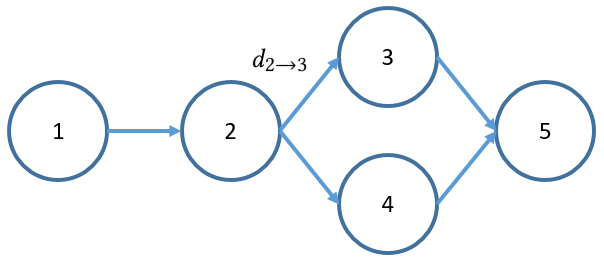
\includegraphics[width=0.3\textwidth]{figures/fork-merge}
	\caption{Example of chain with fork and merge.}
	\label{fig:fork-merge}
\end{figure}

Suppose data consumed by task $2$ must be at most 10 time units old and data consumed by task $5$ must be at most 50 time units old. Our optimization would look like the following:

\begin{align*}
	\text{Given: }& E^{*,*}_i \text{ for each } i \text{ in } 1 \ldots 5\\
	\text{Find: }& P_1, \ldots, P_5\\
	\text{(i.e., Find: }& d_{1 \to 2}, d_{2 \to 3}, d_{2 \to 4}, d_{3 \to 5}, \text{ and } d_{4 \to 5}\text{)}\\
	\text{Minimize: }& \text{Maximum Utilization} \\
	\text{Subject To: }& d_{1 \to 2} \le 10 \\
	\text{ and: }& d_{1 \to 2} + E^{u,max}_2 + d_{2 \to 3} + E^{u,max}_3 + d_{3 \to 5} \le 50 \\
	\text{ and: }& d_{1 \to 2} + E^{u,max}_2 + d_{2 \to 4} + E^{u,max}_4 + d_{4 \to 5} \le 50 \\
	\text{ and: }& \text{each } d_{\star \to \star} > 0
\end{align*}

\noindent From here on out $\star$ is used as a wild card for any valid value that can be used in its place.

Note that this can be easily applied to several pieces of data and is not limited to a single datum. Constraints can be added for several pieces of data and the solution will select the most stringent period required for any one particular data piece.

Below we present the optimization problem for any chain and deadlines. Since we do not know the periods of the tasks during the optimization, we must represent utilization using the provided parameters. We do this using the local deadlines. The optimization problem is as follows:

\begin{align*}
	\text{Given: }& E^{l,min}_i, E^{u,max}_i \text{ for each } i \text{ in } 1 \ldots n\\
	\text{Find: }& d_{i \to j} \text{ for each } \{i,j\} \in E\\
	\text{Minimize: }& U = \sum_{i : \{i,\star\} \in E} \frac{E^{u,max}_i}{P_i} = \sum_{i : \{i,\star\} \in E} \frac{2 \times E^{u,max}_i}{\min(d_{i \to \star}) + E^{l,min}_i} \\
	\text{Subject To: }& \forall k, \sum_{i : \{i,\star\} \in E_k} E^{u,max}_i + \sum_{i : \{i,j\} \in E_k} d_{i \to j} \le D_k \\
	\text{ and: }& \forall{\{i,j\} \in E}, d_{i \to j} > 0
\end{align*}

Note the problem is not linear due to the utilization objective, but the utilization does monotonically increase as any one local deadline decreases within the constraints. As each variable changes the objective in the same manner (no saddles) and the constraints are are simple addition and comparisons, this problem appears to be convex. While we cannot provide an analytical solution for the $n$ task case with this problem, it performs the same optimization as the analytical case would for any $n$.

Given our intuition from the theory evaluation (later) which suggests earlier chain tasks are often assigned higher priority, we extended the optimization problem to be specific to rate-monotonic scheduling by adding additional constraints dictating that the period of each producing task in a chain is less than or equal to the period of its consuming task. Note that this does not always hold in the 3 task scenario depending upon the parameters, but it is a trend we noticed and was a basis for our intuition. The added constraints will cause earlier tasks to have higher priority with the intention of pushing new values through the chain before consuming older ones. The RM-specific formulation is the same as above but with the added constraint:
\begin{align*}
	&\forall{\{i,j\} \in E}, P_{i} \le P_{j} \\
	\implies &\forall{\{i,j\} \in E}, \forall k : \{j,k\} \in E, \frac{d_{i \to j} + E^{l,min}_i}{2} \le \frac{d_{j \to k} + E^{l,min}_{j}}{2}\\
	%\implies &\forall{\{i,j\} \in E}, \forall k : \{j,k\} \in E, d_{i \to j} + E^{l,min}_i \le d_{j \to k} + E^{l,min}_{j}\\
\end{align*}

Other constraints may be added by the designer if desired. For example, in either formulation, if a polling task $T_1$ must run at least every 50 time units as per the Nyquist requirement, an additional constraint could be added: $P_1 \le 50$. Note $P_1$ would have to converted to use the local deadline notation similar to above.

Finally, note that this method works for multiple disconnected task chains. That is, the requirements of each chain can be encoded in the optimization constraints while the objective function remains the utilization of all tasks. An entire system of complex task chains with forks, merges, and multiple data pieces can be simultaneously optimized in a single optimization problem.
	\section{Preemption and Other Job Delays}

While Figure~\ref{fig:3Tasks} depicts task $B$ running without preemption, here we will explain why preemption (or other task delays during execution) do not invalidate our theory.

\begin{theorem}
	Preemption and other job delays do not cause data freshness violations.
\end{theorem}

\begin{proof}
	Assume this is not the case, i.e. that job preemption and other delays cause a freshness miss. Let all preemption and other job delays be denoted by $p$.
	
	Consider any producer ($A$) and consumer ($B$) task pair. Note that the maximum wait scenario in Figure~\ref{fig:2Tasks} holds regardless of the execution time of the second job of task $A$ and regardless of the release time of task $B$. Thus our primary concern in the first execution of task $A$. Note that the first job of task $A$ experiencing preemption produces fresher data, so preemption of the first job does not extend $d_{A \to B}$ either. Hence, preemption of task $A$ or $B$ cannot extend $d_{A \to B}$ as long as the task set is schedulable. Therefore each local deadline is not violated by preemption.
	
	Now consider the intermediate tasks in the chain, which are a part of two, two-task scenarios. If preemption extends a job, its does not affect the first pair as execution time of a consumer is irrelevant. Preemption also does not effect the second pair, as preemption extends the completion time of the job resulting in fresher data local data in the worst-case scenario as described above. Therefore preemption of intermediate jobs does not violate freshness. Any preemption and other delays are experienced entirely within a local constraint, i.e. $p$ in preemption time comes with data $p$ newer than the task's local constraint in worst case.
	
	Since all subcomponents of the freshness bound are not violated by preemption, the end-to-end deadline is not violated by preemption.
\end{proof}

While we have proven preemption will not violate our freshness constraint, it is important to note that preemptability may be key to calculating schedulability. Our solution provides period assignments, which may affect priorities and preemption behavior, hence the post-result schedulability test should be mindful of the preemptability or non-preemptability of the implementation system when determining if the resulting task set is feasible.
	\section{Multiprocessor Systems}

Our formulation extends nicely to multiprocessor systems since we do not make assumptions on how to schedule tasks. The worst case is that all tasks in the chain end up on the same processor which happens to be the exact case we consider. However, no assumptions on task location were made so tasks could be executed on the same or different processors.

Also note that our formulation selects periods for each producing task and is agnostic to the consuming task. For each producer-consumer pair, the period of the producer is chosen so that the produced value is updated within the desired freshness constraint. It does not matter when nor where the consumer task is executed. As long as delays introduced in a multiprocessor system are accounted for in the data delay values, tasks may execute on any processor and still maintain the freshness guarantee.

With this, it is simple to see that the generality of the formulation includes the multiprocessor scenario, and adding processors does not change the correctness of our solution. On the other hand, more processors does help ensure the schedulability of the resulting task set by increasing the resources available in the system and preventing job blocking and preemption. The only change required for use on a multiprocessor system is to use the schedulability test for the multiprocessor algorithm chosen once optimization results are obtained.

Delays in job completion related to multiprocessor execution are not problematic, as shown in our section on preemption and other job execution delays.
	\section{Evaluation}

\subsection{3-Task Theory Evaluation}

For evaluating our three-task theory, we perform four experiments. In the first, we run the tasks on a real-time system and record the miss rate and average freshness of data. Next, we take chains of tasks and a given freshness guarantee, and then check if the produced results are theoretically schedulable. Later, we evaluate how schedulability and utilization may change when altering the desired freshness. Lastly, we examine one task chain and see how the period assignments change when we modify the freshness bound.

For our evaluation we consider uniprocessor systems for simplicity. As described earlier, the evaluation conclusions should largely apply to the multiprocessor systems as well. To test schedulability we use response time analysis for rate monotonic (RM) scheduling and a utilization bound of 1 for earliest deadline first (EDF) scheduling. For our task parameters, we use values from the E3S benchmark\footnote{http://ziyang.eecs.umich.edu/\textasciitilde dickrp/e3s/}. We used all sections of the benchmark, including task sets from the automotive, consumer electronics, networking, office automation, and telecommunications industries.

The task graphs we obtained have between 2 and 10 tasks. To gather as many relevant examples as possible for these special cases, we sometimes combined several serial tasks into one large task, or used several branches of parallel tasks as separate examples for 2-and-3-task evaluations. However, we always included the beginning and ending tasks and some chain from the former to the latter, so that the period values in the benchmark could be used meaningfully. We used WCETs of the first hardware configuration given in the benchmark, and chose BCETs to be half of WCET. We considered communication negligible for evaluation as we global variables between threads of the same process. In total, we collected 26 three-task scenarios and 29 two-task scenarios from the benchmark suite.

For our first experiment, we ran task chains with parameters chosen by our theory on a real system, using a freshness bound of 25\% of the period of the final task so as to have difficult enough chains for meaningful evaluation. We used a Linux testbed\footnote{Ubuntu 14.04, i7-6770HQ CPU, 16GB DDR3 RAM} with either the fixed priority scheduler (SCHED\_FIFO) with priorities set to RM, or the EDF scheduler (SCHED\_DEADLINE). We set up the tasks to run for 99\% of the specified WCET to account for scheduler overhead and context switching. The final task maintains statistics such as average freshness and freshness miss ratio. We ran this for all task sets that passed the respective schedulability test after having parameters selected by our formulation. The average utilization of the task sets was 40.6\% with a low of 1.9\% and a high of 97.4\%. We ran each task set for one minute, which resulted in hundreds to hundreds of thousands of executions of each task. Tasks were all run on the same core with no external loads added.

Under both RM and EDF, all reads by the last task were within the desired freshness bound, i.e. there were no misses, except for far outliers (3-5x the bound) which we discarded as OS, background task, and other outside interferences, as these are far larger than could be reasonably expected. The average percentage of the freshness bound that was consumed before reading a value as well as the average percentage bound consumed for the stalest value were recorded. The top section of Table \ref{table:fresh} summarizes the results. We see that on average the value was well within the maximum bound. Our experiments suggest that RM slightly outperforms EDF when considering average freshness. RM shows the greatest advantages for maximum staleness observed. We believe this is because our 2-and-3-task theory often assigns lower periods, and hence higher priorities, to tasks earlier in the task chain. This may help freshness since producer tasks are executed first which prioritizes pushing newer values though the chain over consuming older values.

\begin{table}[h]
\caption{Comparison of average freshness and miss percentage for task sets under RM and EDF scheduling}
\label{table:fresh}
\begin{center}
	\begin{tabular}{|r|c|c|}
		\hline
		Original Task Set & RM & EDF \\
		\hline
		Freshness Miss Rate (\%) & 0 & 0 \\
		Average Freshness (\% of bound) & 7.8 & 10.3 \\
		Average Max Freshness (\% of bound) & 12.9 & 52.9 \\
		\hline
		Stringent Task Set & RM & EDF \\
		\hline
		Freshness Miss Rate (\%) & 0 & 0 \\
		Average Freshness (\% of bound) & 11.5 & 13.2 \\
		Average Max Freshness (\% of bound) & 26.2 & 81.9 \\
		\hline
	\end{tabular}
\end{center}
\end{table}

The statistics collected in the trial were weighted down by several easily scheduled task sets. To get an idea of how the formulation performed on heavier task sets, we removed task sets where 20\% or less of the bound was consumed on average. In this case the average utilization was 45.2\% with a low of 20.6\% and a high of 83.4\%. We observed the same trend as before where RM outperforms EDF on average, and especially in the maximum staleness metric. The results are shown in the bottom section of Table \ref{table:fresh}.

For our second experiment, we looked at the theoretical schedulability of the task sets. Figure \ref{fig:Schedulability} shows the percentage of task chains which were schedulable using RM or EDF scheduling. The first two sets of bars depict the schedulability percentage when freshness bounds are set equal to the period of the last task in the chain. The second two sets of bars depict the schedulability after we quarter the freshness bound. If the freshness bound is too tight, our formulation will sometimes result in non-positive periods. These cases were included in the evaluation and were considered unschedulable task chains.

\begin{figure}[h]
\centering
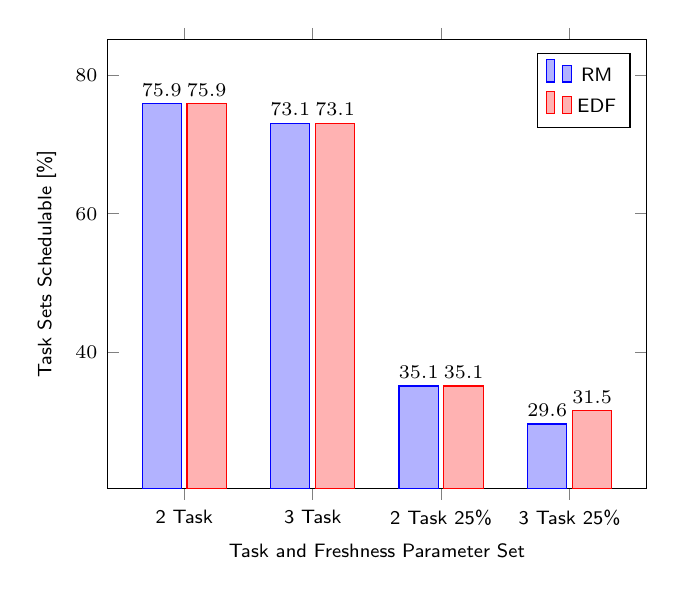
\begin{tikzpicture}[font=\sffamily\scriptsize]
	\begin{axis}[
	ybar,
	enlargelimits=0.2,
	bar width = 0.5cm,
	legend style={legend columns=1},
	legend pos=north east,
	xlabel={Task and Freshness Parameter Set},
	ylabel={Task Sets Schedulable [\%]},
	symbolic x coords={2 Task,3 Task,2 Task 25\%,3 Task 25\%},
	xtick=data,
	nodes near coords,
	nodes near coords align={vertical},
	every node near coord/.append style={color=black, rotate=0, anchor=center,  xshift=0, yshift=5}]
	
	\addplot [forget plot] coordinates {};
	\addplot coordinates {(2 Task,75.9) (3 Task, 73.1) (2 Task 25\%,35.1) (3 Task 25\%,29.6)};
	\addplot coordinates {(2 Task,75.9) (3 Task, 73.1) (2 Task 25\%,35.1) (3 Task 25\%,31.5)};
	
	\legend{RM,EDF}
	\end{axis}
\end{tikzpicture}
\caption{Formulation Schedulability. The first two bar sets show schedulability of task chains with freshness bound equal to period of the last task. The last two bar sets show schedulability when the bound is quartered.}
\label{fig:Schedulability}
\end{figure}

Both schedulers scheduled the same percentage of tasks for the first 3 bar sets and inspection revealed both scheduled the same task chains. The last bar set depicts a task set which showed discrepancy between RM and EDF schedulers, where EDF shows a slight schedulability advantage.

For our third experiment, we choose to repeatedly decrease the freshness bound of each schedulable task set by 10\% from an original freshness bound (equal to the period of the last task in the chain). We then recorded the average utilization and percentage of task chains that are schedulable under EDF. This gives us an idea of the trade-off between freshness and schedulability. The results are charted in the top two lines of Figure \ref{fig:FreshnessChange}. We can see that above about 50\% of the original bound a 10\% decrease in freshness bound results in about 5\% increase in utilization. The areas where utilization decreases (30\% and lower) is due to less task sets being considered, since non-schedulable task chains were omitted from the utilization calculation. We see schedulability is not greatly hindered until we get to around 30\% of the original freshness bound. The primary significance of Figure \ref{fig:FreshnessChange} is that above 30\% of original freshness bound, where the task set stays largely the same, we see only modest increases in utilization when we tighten the freshness bound.

\begin{figure}[h]
\centering
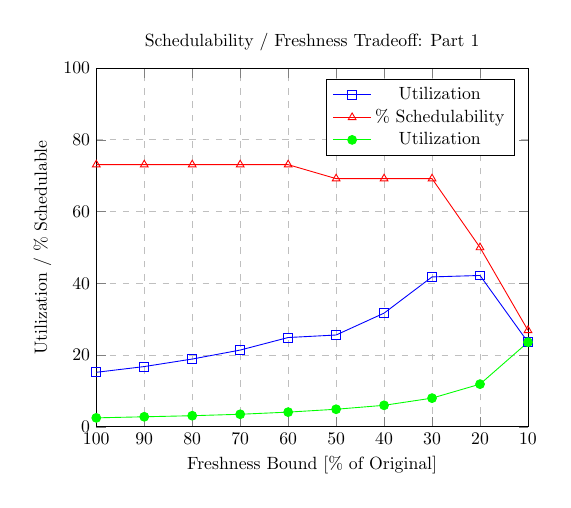
\begin{tikzpicture}[thick,scale=.8, every node/.style={scale=.8}]
\begin{axis}[
title={Schedulability / Freshness Tradeoff: Part 1},
xlabel={Freshness Bound [\% of Original]},
ylabel={Utilization / \% Schedulable},
xmin=10, xmax=100,
ymin=0, ymax=100,
ytick={0,20,40,60,80,100},
xtick={10,20,30,40,50,60,70,80,90,100},
xticklabels={100,90,80,70,60,50,40,30,20,10},
legend pos=north east,
ymajorgrids=true,
xmajorgrids=true,
grid style=dashed,
]

\addplot[
color=blue,
mark=square,
]
coordinates {
	(100,23.6)(90,42.2)(80,41.8)(70,31.7)(60,25.6)(50,24.9)(40,21.4)(30,18.9)(20,16.8)(10,15.2)
};

\addplot[
color=red,
mark=triangle,
]
coordinates {
	(100,26.9)(90,50)(80,69.2)(70,69.2)(60,69.2)(50,73.1)(40,73.1)(30,73.1)(20,73.1)(10,73.1)
};

\addplot[
color=green,
mark=*,
]
coordinates {
	(100,23.6)(90,11.9)(80,8)(70,6)(60,4.9)(50,4.1)(40,3.5)(30,3.1)(20,2.8)(10,2.5)
};

\legend{Utilization,\% Schedulability, Utilization}
\end{axis}
\end{tikzpicture}
\caption{Schedulability, Utilization vs. Freshness.}
\label{fig:FreshnessChange}
\end{figure}

Next we modified the previous experiment by performing the evaluation only on those chains which are schedulable at 10\% of the original freshness bound, to prevent noise due to the differences in the schedulable task chains. In the bottom line of Figure \ref{fig:FreshnessChange} we see a more intuitive curve. It is lower because more difficult chains were not schedulable with very low freshness bounds. Note that a 10\% reduction does not change utilization much if above 50\% of the original freshness bound. We see again that utilization is more greatly affected when below 30\% of the original freshness bound.

\iffalse
\begin{figure}[h]
	\centering
	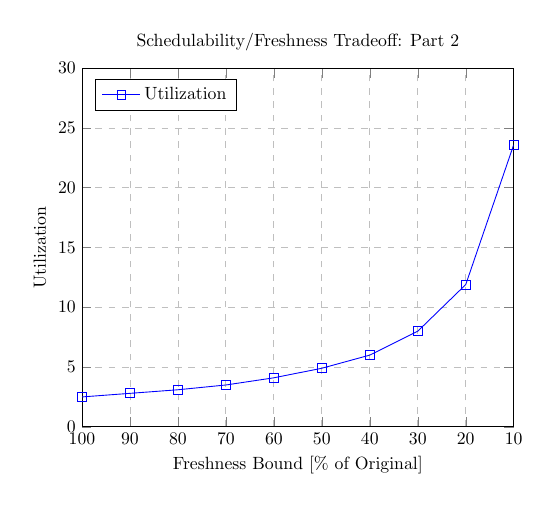
\begin{tikzpicture}[thick,scale=.8, every node/.style={scale=.8}]
	\begin{axis}[
	title={Schedulability/Freshness Tradeoff: Part 2},
	xlabel={Freshness Bound [\% of Original]},
	ylabel={Utilization},
	xmin=10, xmax=100,
	ymin=0, ymax=30,
	ytick={0,5,10,15,20,25,30},
	xtick={10,20,30,40,50,60,70,80,90,100},
	xticklabels={100,90,80,70,60,50,40,30,20,10},
	legend pos=north west,
	ymajorgrids=true,
	xmajorgrids=true,
	grid style=dashed,
	]
	
	\addplot[
	color=blue,
	mark=square,
	]
	coordinates {
		(100,23.6)(90,11.9)(80,8)(70,6)(60,4.9)(50,4.1)(40,3.5)(30,3.1)(20,2.8)(10,2.5)
	};
	
	\legend{Utilization}
	\end{axis}
	\end{tikzpicture}
	\caption{Freshness vs. Utilization. Result for task chains that remain schedulable even with a freshness bound 10\% of the consuming task's period.}
	\label{fig:FreshnessChangeControlled}
\end{figure}
\fi

For our fourth experiment, we chose a three task chain which was schedulable with freshness bound of 10\% of the period of the last task. This chain was from the automotive industry. We then calculated the periods of the input tasks according to our theory in increments of 10\% of the original freshness bound. We'll name our tasks in the chain as $A \to B \to C$. In this case, task $A$ has a WCET of $50$, task $B$ a WCET of $155$, and task $C$ a period and WCET of $15000$ and $50$ milliseconds respectively. BCETs were set to half of WCET. How the assigned periods of tasks $A$ and $B$ change to reflect the change in freshness bound is displayed in Figure \ref{fig:TaskSet4}. We see that changes in freshness causes linear changes in the periods of both tasks to account for the new bound.

\begin{figure}[h]
	\centering
	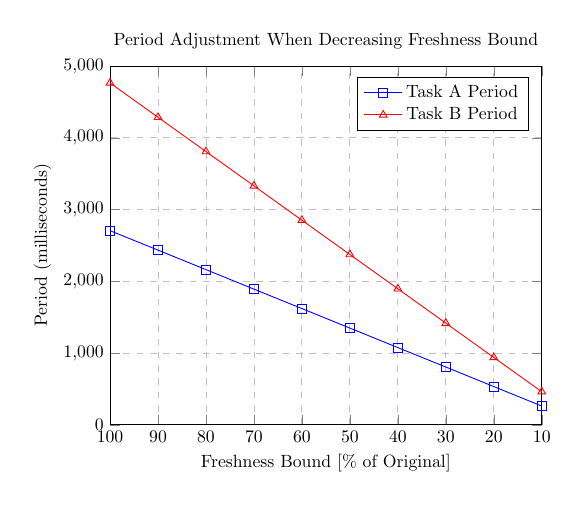
\begin{tikzpicture}[thick,scale=.8, every node/.style={scale=.8}]
	\begin{axis}[
	title={Period Adjustment When Decreasing Freshness Bound},
	xlabel={Freshness Bound [\% of Original]},
	ylabel={Period (milliseconds)},
	xmin=10, xmax=100,
	ymin=0, ymax=5000,
	ytick={0,1000,2000,3000,4000,5000},
	xtick={10,20,30,40,50,60,70,80,90,100},
	xticklabels={100,90,80,70,60,50,40,30,20,10},
	legend pos=north east,
	ymajorgrids=true,
	xmajorgrids=true,
	grid style=dashed,
	]
	
	\addplot[
	color=blue,
	mark=square,
	]
	coordinates {
		%(10,0.34)(20,0.66)(30,0.99)(40,1.30)(50,1.62)(60,1.94)(70,2.26)(80,2.58)(90,2.89)(100,3.21)
		(100,262)(90,534)(80,806)(70,1077)(60,1349)(50,1621)(40,1892)(30,2164)(20,2436)(10,2707)
	};
	
	\addplot[
	color=red,
	mark=triangle,
	]
	coordinates {
		%(10,0.23)(20,0.41)(30,0.59)(40,0.77)(50,0.95)(60,1.13)(70,1.31)(80,1.49)(90,1.67)(100,1.85)
		(100,462)(90,940)(80,1418)(70,1897)(60,2375)(50,2853)(40,3332)(30,3810)(20,4288)(10,4767)
	};
	
	\legend{Task A Period, Task B Period}
	\end{axis}
	\end{tikzpicture}
	\caption{Freshness vs. Periods. Using one task chain that is schedulable with a freshness bound at 10\% of task $C$'s period, we plot how our formulation assigns periods tasks $A$ and $B$ to maintain freshness.}
	\label{fig:TaskSet4}
\end{figure}

\subsection{Optimization Formulation Evaluation}

To evaluate the optimization formulation we implemented the described optimization problems in MATLAB. In our figures we will denote the general formulation as ``G-'' and the RM-targeting formulation as ``R-'' followed by the scheduler used. For example, G-RM denotes data using solutions from the general formulation ran under a RM scheduler.

For each chain length, we randomly generated tasks with between 1 and 5 units of work for their BCET, and added another 1 to 5 to the BCET to determine the WCET. We then generated an end-to-end deadline equal to the sum of the task WCETs multiplied by a random integer between 3 and 10, in order to add slack to the system that depends on the number of tasks and their execution lengths so that chain lengths and WCETs do not adversely affect the results. All random variables were drawn from a uniform distribution. We used the same necessary and sufficient schedulability uniprocessor tests for RM and EDF as before. Figure \ref{fig:OptimizationOptimizationByChainLength} depicts the schedulability of the generated task sets. Each bar represents the percentage of 1000 generated task sets that were schedulable. Note the same 1000 task sets were used for each formulation-scheduler combination.

\begin{figure}[h]
	\centering
	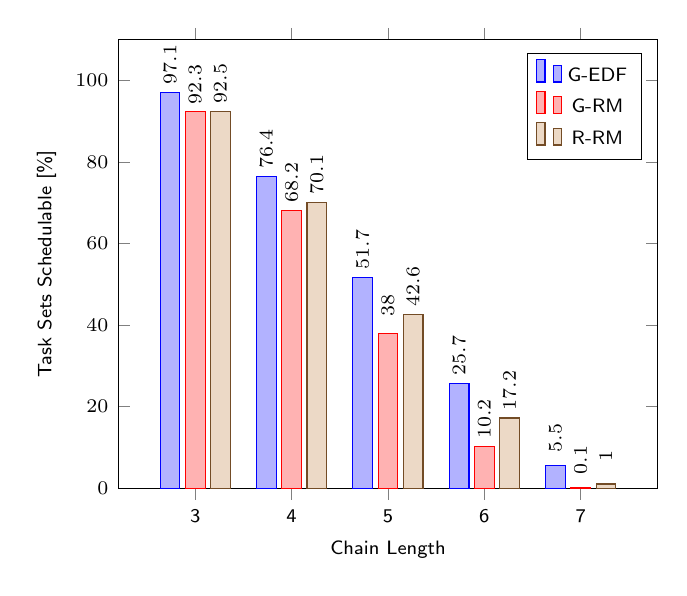
\begin{tikzpicture}[font=\sffamily\scriptsize]
	\begin{axis}[
	ybar,
	enlargelimits=0.2,
	enlarge y limits={upper=0},
	bar width = 0.25cm,
	legend style={legend columns=1},
	legend pos=north east,
	xlabel={Chain Length},
	ylabel={Task Sets Schedulable [\%]},
	symbolic x coords={3,4,5,6,7},
	ymin=0, ymax=100,
	xmin=3, xmax=7,
	xtick=data,
	nodes near coords,
	nodes near coords align={vertical},
	every node near coord/.append style={color=black, rotate=90, anchor=center, xshift=10, yshift=0}]
	
	\addplot [forget plot] coordinates {};
	\addplot coordinates {(3,97.1) (4, 76.4) (5,51.7) (6,25.7) (7,5.5)};
	\addplot coordinates {(3,92.3) (4, 68.2) (5,38.0) (6,10.2) (7,0.1)};
	\addplot coordinates {(3,92.5) (4, 70.1) (5,42.6) (6,17.2) (7,1.0)};
	
	\legend{G-EDF,G-RM,R-RM}
	\end{axis}
	\end{tikzpicture}
	\caption{Schedulability of Optimization Results with Differing Chain Lengths.}
	\label{fig:OptimizationOptimizationByChainLength}
\end{figure}

We see that EDF performs more favorably in terms of schedulability. However, we do see a small improvement in RM schedulability when we use our RM-targeted formulation. This improvement seems to increase with chain length.

\iffalse
\begin{figure}[h]
	\centering
	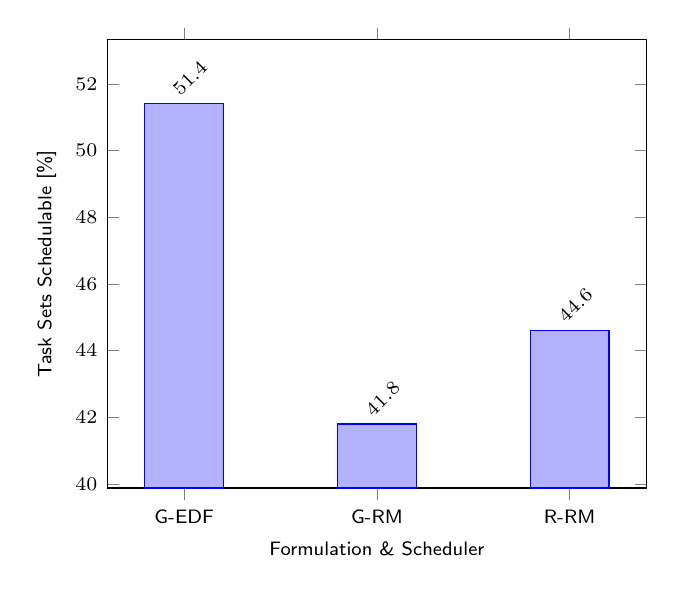
\begin{tikzpicture}[font=\sffamily\scriptsize]
	\begin{axis}[
	ybar,
	enlargelimits=0.2,
	bar width = 1cm,
	legend style={at={(0.5,1.15)},
		anchor=north,legend columns=-1},
	xlabel={Formulation \& Scheduler},
	ylabel={Task Sets Schedulable [\%]},
	symbolic x coords={G-EDF,G-RM,R-RM},
	xtick=data,
	nodes near coords,
	nodes near coords align={vertical},
	every node near coord/.append style={color=black, rotate=45, anchor=center, xshift=8, yshift=5}]
	
	\addplot [forget plot] coordinates {};
	\addplot coordinates {(G-EDF, 51.4) (G-RM,41.8) (R-RM,44.6)};
	
	\end{axis}
	\end{tikzpicture}
	\caption{Schedulability of Optimization Results with Mixed Chain Lengths Between 3 and 7 Inclusive.}
	\label{fig:OptimizationOptimizationRandomChains}
\end{figure}
\fi

%Using the same generation methods as above but instead randomly generating chain lengths between 3 and 7, we saw the schedulability depicted in Figure \ref{fig:OptimizationOptimizationRandomChains}.

To show that our method is applicable to longer chain lengths and to analyze the scaling ability of the method according to the task set, we ran the above optimization and analysis but with a harder and easier task sets. More precisely, we kept the same task set as depicted in Figure \ref{fig:OptimizationOptimizationByChainLength} but with the end-to-end freshness deadline either halved (twice as hard) or doubled (half as hard). The results of the latter are shown in Figure~\ref{fig:OptimizationOptimizationByChainLengthEasy}.

\iffalse
\begin{figure}[h]
	\centering
	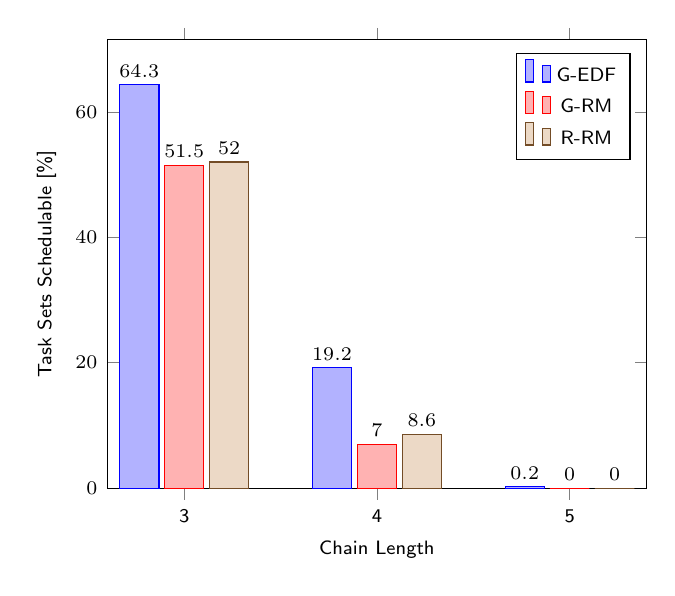
\begin{tikzpicture}[font=\sffamily\scriptsize]
	\begin{axis}[
	ybar,
	enlargelimits=0.2,
	enlarge y limits={upper=0},
	bar width = 0.5cm,
	legend style={legend columns=1},
	legend pos=north east,
	xlabel={Chain Length},
	ylabel={Task Sets Schedulable [\%]},
	symbolic x coords={3,4,5},
	ymin=0, ymax=65,
	xmin=3, xmax=5,
	xtick=data,
	nodes near coords,
	nodes near coords align={vertical},
	every node near coord/.append style={color=black, rotate=0, anchor=center, xshift=0, yshift=5}]
	
	\addplot [forget plot] coordinates {};
	\addplot coordinates {(3,64.3) (4, 19.2) (5,0.2)};
	\addplot coordinates {(3,51.5) (4, 7.0) (5,0.0)};
	\addplot coordinates {(3,52.0) (4, 8.6) (5,0.0)};
	
	\legend{G-EDF,G-RM,R-RM}
	\end{axis}
	\end{tikzpicture}
	\caption{Schedulability of Optimization Results with Differing Chain Lengths, with deadlines halved. This approximates a twice as difficult task set.}
	\label{fig:OptimizationOptimizationByChainLengthHard}
\end{figure}
\fi

\begin{figure}[h]
	\centering
    %\begin{adjustbox}{width=0.85\textwidth}
	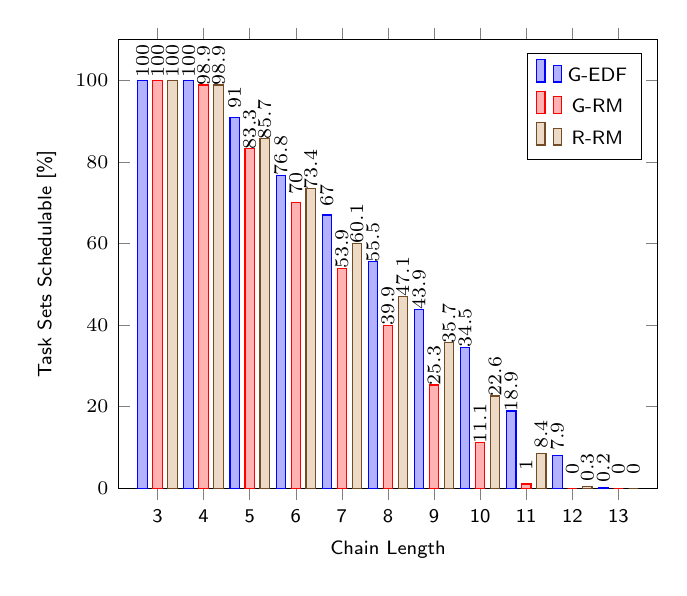
\begin{tikzpicture}[font=\sffamily\scriptsize]
	\begin{axis}[
	ybar,
	enlargelimits=0.2,
    enlarge x limits={abs=0.5cm},
    enlarge y limits={upper=0},
	bar width = 0.12cm,
	legend style={legend columns=1},
	legend pos=north east,
	xlabel={Chain Length},
	ylabel={Task Sets Schedulable [\%]},
	symbolic x coords={3,4,5,6,7,8,9,10,11,12,13},
	ymin=0, ymax=100,
	xmin=3, xmax=13,
	xtick=data,
	nodes near coords,
	nodes near coords align={vertical},
	every node near coord/.append style={color=black, rotate=90, anchor=center, xshift=7, yshift=0}]
	
	\addplot [forget plot] coordinates {};
	\addplot coordinates {(3,100.0) (4, 100.0) (5,91.0) (6,76.8) (7,67.0) (8,55.5) (9,43.9) (10,34.5) (11,18.9) (12,7.9) (13,0.2)};
	\addplot coordinates {(3,100.0) (4, 98.9) (5,83.3) (6,70.0) (7,53.9) (8,39.9) (9,25.3) (10,11.1) (11,1.0) (12,0.0) (13,0.0)};
	\addplot coordinates {(3,100.0) (4, 98.9) (5,85.7) (6,73.4) (7,60.1) (8,47.1) (9,35.7) (10,22.6) (11,8.4) (12,0.3) (13,0.0)};
	
	\legend{G-EDF,G-RM,R-RM}
	\end{axis}
	\end{tikzpicture}
        %\end{adjustbox}
	\caption{Schedulability of Optimization Results with Differing Chain Lengths: Deadlines Doubled.}
	\label{fig:OptimizationOptimizationByChainLengthEasy}
\end{figure}

We can see that the trend remains about linear in schedulability after the modification. Similar scaling was seen in the more difficult task set but the figure is omitted due to space considerations. These experiments suggest that the formulation's schedulability generally scales inversely with chain length. There is no chain length from our trials that causes the schedulability to unexpectedly drop. It appears that our formulation can handle approximately twice the chain length for each halving in difficulty and vice versa, with some small losses due to pessimism.

In our final evaluation we again referenced the E3S benchmark to evaluate real-world performance with multiple chain lengths. We chose chains that all three formulations could schedule. We ran the chains and collected freshness data as we did in the three-task theory evaluation. The results are summarized in the Table \ref{table:freshess_e3s}.

\begin{table}[h]
	\caption{Comparison of freshness for task chains under RM or EDF scheduling using results from the general or RM-specific formulation.}
	\label{table:freshess_e3s}
	\begin{center}
		\begin{tabular}{|r|c|c|c|}
			\hline
			& G-EDF & G-RM & RM-RM \\
			\hline
			Average Freshness (\% of bound) & 13.73 & 4.77 & 4.77 \\
			Average Max Freshness (\% of bound) & 56.20 & 33.75 & 31.89 \\
			\hline
		\end{tabular}
	\end{center}
\end{table}

RM scheduling provided better average and maximum staleness when executing the results from either optimization, further supporting that for real-world task sets similar to the E3S benchmark, RM provides greater freshness than EDF.

Overall, our optimization formulation seems adequate for short to moderate chain lengths. We suspect that many real-life systems use chain lengths within the evaluated ranges, including all of the E3S benchmark chains. As far as optimization efficiency, the optimization problem finished on average in less than a second. This suggests that the scaling of the optimization problem would not be a limiting factor in the use of our system.

	\section{Discussion}

We note several issues with this approach. For one, it generalizes for any scheduling algorithm. Given information about the scheduling algorithm, prioritization, and preemptability, one could likely produce parameters that result in lower utilization. For many schedulers this would mean larger periods for our input tasks than presented in our solution.

The most important limitation to note, as mentioned several times already, is that this method does not guarantee the schedulability of the task set. This is due to its scheduler agnosticism. However, this is easily remedied by scheduler-specific schedulability tests. A weak, universal, necessary assessment would be to check if the utilization is less than 1, since we are considering a uniprocessor system. If the particular value produced by this method is unschedulable, there may or may not exist other parameters that schedule the task set while ensuring freshness for a given scheduler. This becomes particularly difficult if extended to multicore systems.

It may be possible to extend this model further to even more tasks. Using the same notation as used for the three task model, one could craft complex minimization problems for a given number of tasks. The primary challenge would then be solving increasingly difficult optimization problems. It may be possible to generalize this method to $n$ tasks but this has not yet been pursued.
	\section{Related Work}
Others have investigated proper period selection for tasks. However, most opt to consider a specific scheduler or other assumptions about the task set, or don't consider data freshness as the end goal. [To be expanded]
	\section{Conclusion}

In this paper we considered the freshness of data consumed by tasks within a periodic task system. We aimed to select the periods of input tasks in order to ensure the freshness of data consumed later chain tasks. Without assumptions regarding the scheduler, we proved upper bounds on the periods of tasks in order to ensure the freshness of data through chains of tasks of length two and three for uniprocessor systems. We then extended the theory to an optimization problem suitable for any chain length and configuration.
	
	%%
	%% Bibliography
	%%
	
	%% Either use bibtex (recommended), 
	
	\bibliographystyle{ACM-Reference-Format}
	%\bibliography{sigproc}
	\bibliography{references}
	
	%% .. or use the thebibliography environment explicitely
\end{document}

